\label{sec:introdutction}
In recent years, with the development of the hardware and algorithms, the capabilities of a single agent have been significantly improved.
To further expand the capabilities of intelligent robots, using several robots can accelerate many tasks, such as localization, exploration, and mapping.
As simultaneous localization and mapping(SLAM) is an essential component in many tasks, it is important to do SLAM across different robots in many multi-agent applications.
The camera is a widely used sensor in SLAM for its rich information and low cost. The previous work \cite{Cieslewski:20187ee} proposes a data-efficient decentralized SLAM(DSLAM) system based on the stereo camera.
Especially, because it is simpler to deploy and does not require calibration, the monocular camera has become a hot topic in academic research. We aim to build up a monocular visual-based DSLAM in this work.

The goal of DSLAM is to share the maps and trajectories among the robots in a communication-constrained scenario. Also, because the communication is limited, there is not a central node that obtains all the sensor information from each agent, so that we need to design a specially optimized communication mechanism. There are three kinds of data need to be shared among agents: 1) the trajectory of each robot for merging, 2) the encoded information of place recognition for the coarse matching of inter-robot tracks, and 3) the details of the matched frame for inter-robot pose calculation and trajectory merging. The previous work \cite{Cieslewski:20187ee} uses ORB feature-point based method to estimate the trajectory from the sequence of the stereo camera, and use NetVLAD \cite{Arandjelovic:2017997} to do place recognition. Once the coarse matching of inter-robot tracks based on the NetVLAD succeeds, the ORB feature points of the corresponding frames are communicated for fine-grained inter-robot trajectory merging. However, \cite{Cieslewski:20187ee} needs to calculate the ORB feataure extraction and matching algorithm as well as the CNN-based NetVLAD algorithm simultaneously on the embedded system. These two algorithms both consume a large amount of computation and storage, and pose a great challenge to DSLAM on the embedded system. The DSLAM frame in \cite{Cieslewski:20187ee} is illustrated in \cref{fig:all_pre}.

\begin{figure*}[thb]
    \begin{minipage}[t]{0.5\linewidth}  
    \centering
    \subfigure[DSLAM in \cite{Cieslewski:20187ee}] {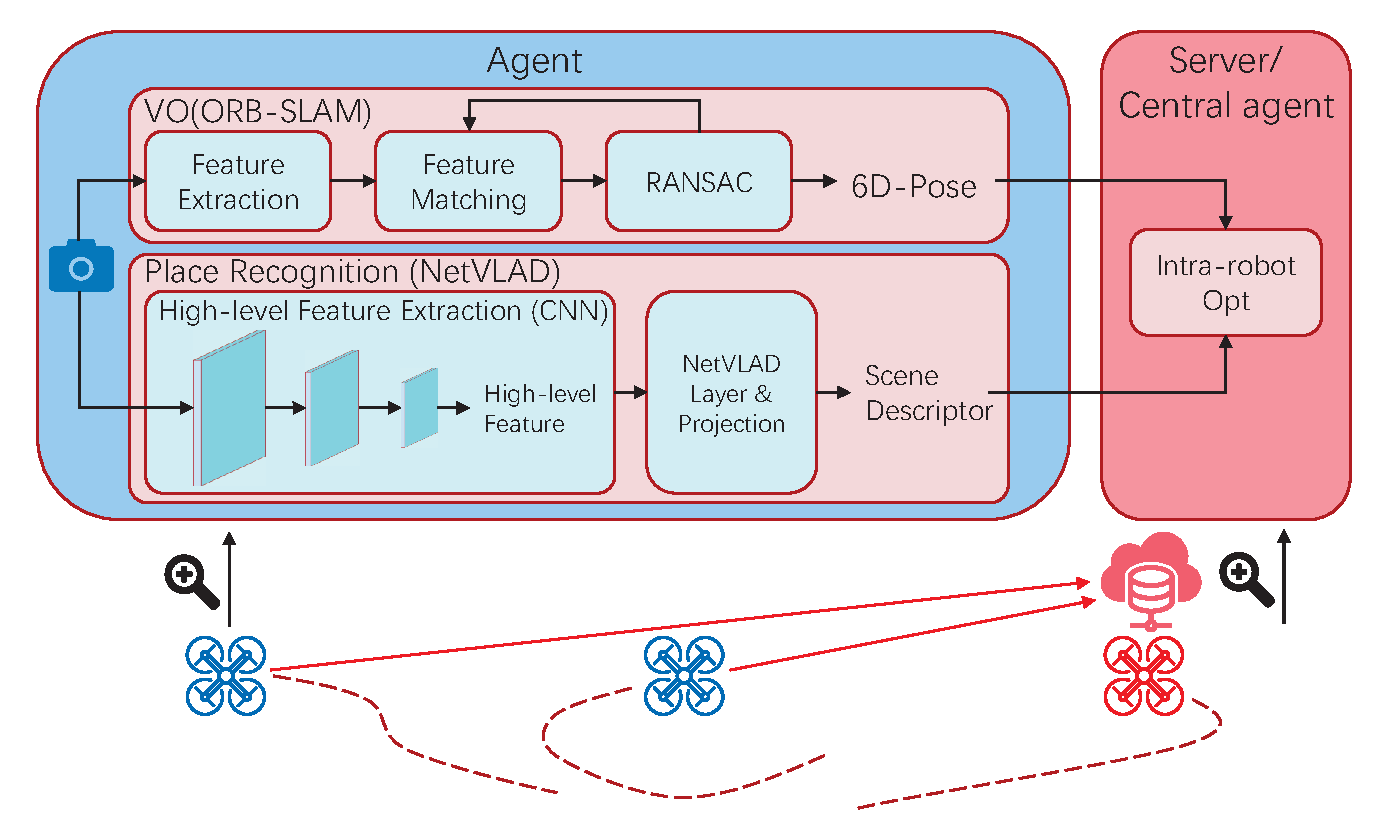
\includegraphics[width=0.95\textwidth]{fig/overview_pre.eps}\label{fig:all_pre}}
    \end{minipage}
    \begin{minipage}[t]{0.5\linewidth}  
    \centering  
    \subfigure[Our hardware-software co-design DSLAM.] {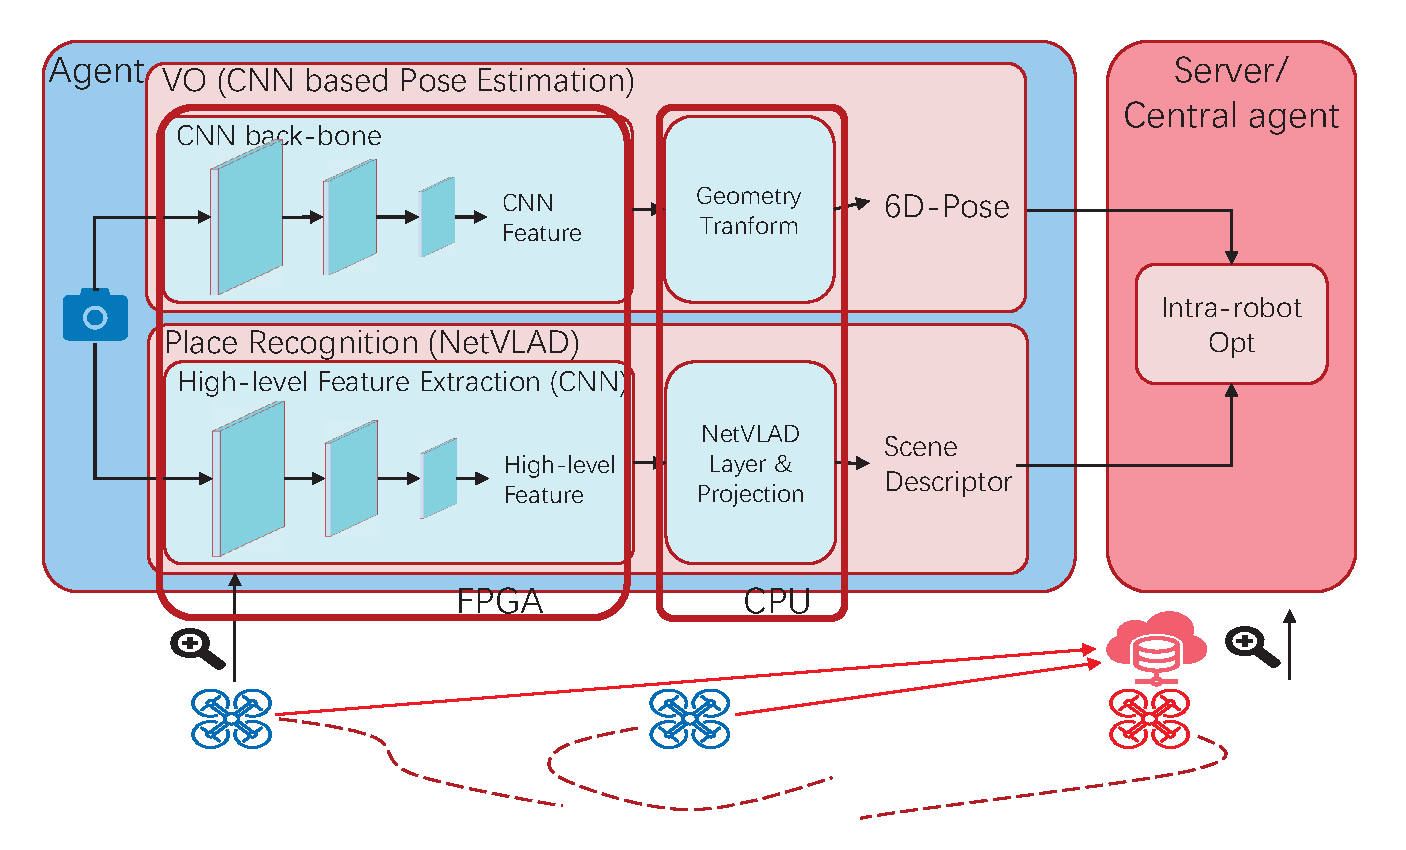
\includegraphics[width=0.95\linewidth]{fig/overview_us.eps}\label{fig:all_us}} 
    \end{minipage}
    \caption{Overview of the DSLAM in \cite{Cieslewski:20187ee} and our hardware-software co-design DSLAM. Each agent (blue drones) will send the result of 6-D pose estimation and scene descriptor to a server or a central agent (red server or drone in figure) to do inter-robot place recognition and optimization. We use CNN instead of feature points to do pose estimation so that we can use CNN accelerator to speed up the whole process.}
\label{fig:overview}
\end{figure*}


With the development of neural networks in recent years, many CNN-based algorithms can also be applied to DSLAM systems. With the help of CNN, we can reconstruct the depth and pose with the absolute scale from the monocular camera. Monocular systems are much easier to deploy than binocular systems. 
The tracking based on CNN can be made more robust, as the CNN-predicted depth and pose does not suffer from the accumulated errors from previous frames, as CNN processes on each pair of two frames individually \cite{Tateno:2017776}. As CNN is a versatile and widely researched method for image processing, it is easy to use the same network structure for many other tasks rather than depth or pose estimation, such as object detection \cite{liu2016ssd} and semantic segmentation\cite{long2015fully}.
Last but not least, CNN's computational structure is uniform and can be individually optimized when resources are limited on embedded systems such as embedded GPU\cite{mao2018towards} and embedded FPGA\cite{Yu:2018:IDC:3299999.3283452,Tech:2019360}. Xilinx DPU\cite{Tech:2019360} is one of state-of-the-art FPGA-based CNN accelerators, and is used in this work.

Though DSLAM system can benefit from the development of CNN, the fully CNN-based DSLAM system faces several key issues: 1) The DSLAM system needs to run multiple CNNs simultaneously for multitasking. The requirement of huge computing resources brings a challenge to real-time implementation. 2) Due to the lack of feature point extraction, we need to explore new data-efficient communication mechanism for inter-robot trajectory merging.

To solve the problems mentioned above, we propose a hardware-software co-design DSLAM framework with the following contributions. The proposed DSLAM framework is illustrated in \cref{fig:all_us}:

\begin{itemize}
\item To the best of our knowledge, this work is the first to implement all components of monocular DSLAM with CNN. We adopt Depth-VO-Feat \cite{Zhan:2018e92} in DSLAM system to estimate the pose from the input monocular camera. We use the same method of NetVLAD in \cite{Cieslewski:20187ee} to do place recognition.
\item We use Xilinx DPU to accelerate the DSLAM system on embedded systems. We use fixed-point fine tune method to transformed the original floating-point Depth-VO-Feat model to fixed-point for deploying on Xilinx DPU. The accuracy of the fixed-point model is even better with the floating-point model.
\item We communicate the down sampled images of corresponding matched frames for inter-robot trajectory merging, so that we can also use Depth-VO-Feat and the accelerator.
\end{itemize}
    
   
The rest part of this article is orgnized as follows. \Cref{sec:background} will give the basic idea of CNN based methods and the hardware architecture of embedded FPGA. \Cref{sec:hardsoft} will detail the implementation of our hardware-software co-design DSLAM system. The experiment result will be given in \Cref{sec:experiment}. \Cref{sec:conclusion} will conclude this paper.